\documentclass[11pt,a4paper]{article}
\usepackage[T1]{fontenc}
\usepackage[utf8]{inputenc}
\usepackage{lmodern}
\usepackage{textcomp}
\usepackage[left=1.8cm,right=1.8cm,top=3.0cm,bottom=2.2cm,headheight=36pt,headsep=12pt]{geometry}
\usepackage{multicol}
\usepackage{xcolor}
\usepackage{fancyhdr}\usepackage{tikz}
\usepackage{graphicx}
\usepackage{array}
\usepackage{amsmath,amssymb}
\usepackage{setspace}
\usepackage{longtable}
\graphicspath{{../}}
\definecolor{ygreen}{RGB}{46,139,87}\definecolor{dgreen}{RGB}{28,90,56}
\renewcommand{\normalsize}{\fontsize{10.9}{13.4}\selectfont}
\renewcommand{\familydefault}{\rmdefault}
\setlength{\parindent}{0pt}
\setlength{\columnsep}{0.8cm}
\setlength{\columnseprule}{0.4pt}
\setlength{\multicolsep}{3pt plus 1pt minus 1pt}
\renewcommand{\textsubscript}[1]{\ensuremath{_{\text{\fontsize{8}{8}\selectfont #1}}}}
\renewcommand{\textsuperscript}[1]{\ensuremath{^{\text{\fontsize{8}{8}\selectfont #1}}}}
\newcommand{\qn}[1]{\textbf{\fontsize{11.5}{13}\selectfont #1}}
\newcommand{\qsep}{\par\vspace{13pt}}
\newcommand{\fwrule}{\par\vspace{5pt}\noindent\rule{\linewidth}{1.4pt}\par\vspace{7pt}}
\newsavebox{\fitb}
\newcommand{\fitbox}[1]{\sbox{\fitb}{#1}\ifdim\wd\fitb>\linewidth\resizebox{\linewidth}{!}{\usebox{\fitb}}\else\usebox{\fitb}\fi}
\newcommand{\diqqat}[1]{\par\smallskip\noindent\textbf{Diqqat!} #1\par\medskip}
\newcommand{\javob}{\par\nopagebreak[4]\smallskip\noindent\textbf{Javob:} \rule[-2pt]{7.5cm}{0.4pt}\par\smallskip\noindent\textbf{Diqqat!} Javobingizni javoblar varaqasiga ko`chirib yozing.\par\medskip}
\pagestyle{fancy}
\fancyhf{}
\renewcommand{\headrulewidth}{1.6pt}\renewcommand{\headrule}{{\color{ygreen}\hrule height 1.6pt width\headwidth}}
\newcommand{\hdrlogo}{
\begin{tikzpicture}[baseline=0pt]\fill[ygreen,rounded corners=3pt] (0,0) rectangle (0.95,0.95);\node[white,font=\fontsize{24}{26}\bfseries\selectfont] at (0.475,0.47){K};\node[anchor=west,font=\fontsize{16}{18}\bfseries\selectfont,text=dgreen] at (1.15,0.66){KIMYO};\node[anchor=west,font=\footnotesize\scshape,text=gray] at (1.15,0.2){Milliy sertifikat\ \ 2026};\end{tikzpicture}}
\newcommand{\hdrpill}[1]{\begin{tikzpicture}[baseline=0pt]\node[fill=ygreen,text=white,rounded corners=8pt,inner xsep=10pt,inner ysep=5pt,font=\fontsize{13}{15}\bfseries\selectfont] at (0,0.475){#1};\end{tikzpicture}}
\fancyhead[L]{\hdrlogo}
\fancyhead[R]{\hdrpill{1-variant}}

\fancyfoot[C]{\thepage}
\fancypagestyle{first}{\fancyhf{}\renewcommand{\headrulewidth}{1.6pt}\renewcommand{\headrule}{{\color{ygreen}\hrule height 1.6pt width\headwidth}}\fancyhead[L]{\hdrlogo}\fancyhead[R]{\hdrpill{1-variant}}\fancyfoot[C]{\thepage}}
\begin{document}
\normalsize
\thispagestyle{first}
\noindent\textit{Davriy jadvaldan foydalanish mumkin.}
\par\smallskip
\begin{multicols}{2}
\noindent\qn{1.} Jadvalda nuklidlarning proton soni (\textit{Z}) va massa soni (A) berilgan:
\begin{center}
\renewcommand{\arraystretch}{1.15}
\fitbox{\begin{tabular}{|c|c|c|}\hline
\textbf{Nuklid} & \textbf{\textit{Z}} & \textbf{A} \\ \hline
\textit{X} & 6 & 12 \\ \hline
\textit{Y} & 6 & 14 \\ \hline
T & 7 & 12 \\ \hline
\textit{U} & 7 & 13 \\ \hline
\textit{V} & 6 & 13 \\ \hline
\end{tabular}}
\end{center}
\textit{X} nuklidning nechta izotopi jadvalda keltirilgan?

\noindent A)~\textsl{3} \hfill B)~\textsl{4} \hfill C)~\textsl{1} \hfill D)~\textsl{2}\par
\qsep
\noindent\qn{2.} KMnO\textsubscript{4} tarkibida Mn ning oksidlanish \textbf{darajasini aniqlang.}

\noindent A)~\textsl{+3 va +5} \hfill B)~\textsl{+7} \hfill C)~\textsl{$-$2} \hfill D)~\textsl{+4}\par
\qsep
\noindent\qn{3.} CH\textsubscript{3}--C$\equiv$CH molekulasida sp\textsuperscript{3} gibridlangan uglerod atomlari nechta?

\noindent A)~\textsl{2} \hfill B)~\textsl{3} \hfill C)~\textsl{1} \hfill D)~\textsl{4}\par
\qsep
\noindent\qn{4.} Quyidagi zarrachalardan qaysilari neon atomi bilan izoelektron? 1) Ca\textsuperscript{2+}; 2) F\textsuperscript{$-$}; 3) Al\textsuperscript{3+}; 4) Li\textsuperscript{+}

\noindent A)~\textsl{2, 3} \hfill B)~\textsl{1, 3} \hfill C)~\textsl{1, 2} \hfill D)~\textsl{2, 3, 4}\par
\qsep
\noindent\qn{5.} Brom (\textit{Z} = 35) atomining tashqi energetik pog`onasidagi elektronlar \textbf{sonini aniqlang.}

\noindent A)~\textsl{8} \hfill B)~\textsl{6} \hfill C)~\textsl{7} \hfill D)~\textsl{9}\par
\qsep
\noindent\qn{6.} 100 g 20\% li NaCl eritmasiga 25 g NaCl qo`shib eritildi, so`ngra eritma 100 g suv bilan suyultirildi. Hosil bo`lgan eritmadagi tuzning massa \textbf{ulushini (\%) aniqlang.}

\noindent A)~\textsl{10} \hfill B)~\textsl{36} \hfill C)~\textsl{22,5} \hfill D)~\textsl{20}\par
\qsep
\noindent\qn{7.} Quruq havo tarkibi diagrammada keltirilgan.
\begin{center}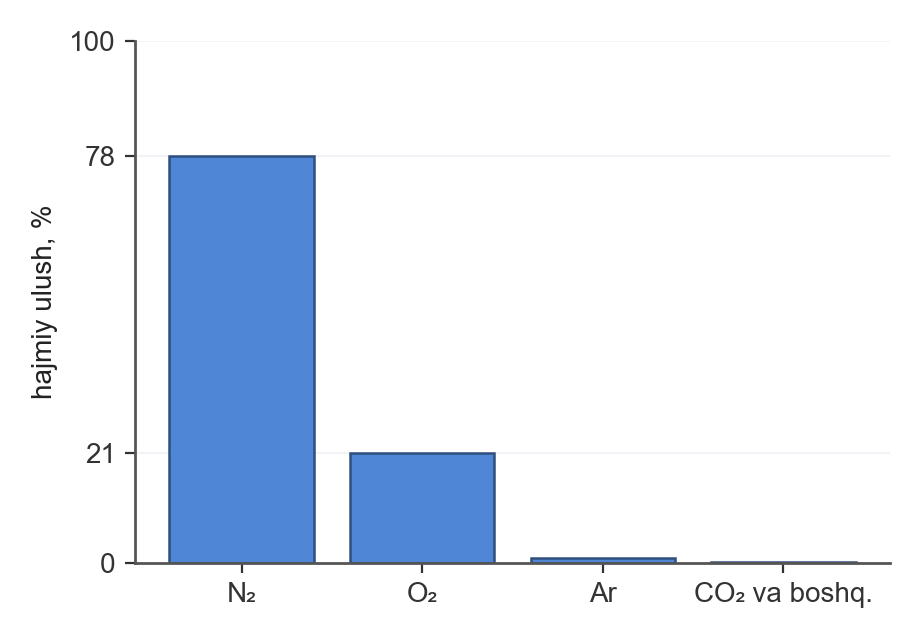
\includegraphics[width=0.86\linewidth]{rasmlar/gen/ai_v01_0.png}\end{center}
100 l (n.sh.) havo tarkibidagi kislorod \textbf{hajmini (l) toping.}

\noindent A)~\textsl{78} \hfill B)~\textsl{42} \hfill C)~\textsl{10,5} \hfill D)~\textsl{21}\par
\qsep
\noindent\qn{8.} Na\textsubscript{2}CO\textsubscript{3} eritmasida gidrolizlanish darajasini oshirish uchun qaysi usullar qo`llanadi? 1) NaOH eritmasi qo`shish; 2) HCl qo`shish; 3) qattiq Na\textsubscript{2}CO\textsubscript{3} qo`shib, konsentratsiyani oshirish; 4) sovitish

\noindent A)~\textsl{1, 3} \hfill B)~\textsl{2} \hfill C)~\textsl{2, 3} \hfill D)~\textsl{2, 4}\par
\qsep
\noindent\qn{9.} Zn va Al aralashmasi tarkibida Al ning mol miqdori Zn nikidan 2/1 marta ko`p. Aralashmaning massasi 23,8 g. Aralashmaning zichligi 5,2 g/sm\textsuperscript{3} ga teng. Ajralgan vodorod \textbf{miqdorini (mol) hisoblang.}

\noindent A)~\textsl{1,6} \hfill B)~\textsl{0,8} \hfill C)~\textsl{0,4} \hfill D)~\textsl{0,6}\par
\qsep
\noindent\qn{10.} 25 g CuSO\textsubscript{4}$\cdot$5H\textsubscript{2}O 100 g suvda eritildi. Eritmadagi tuzning massa \textbf{ulushini (\%) aniqlang.}

\noindent A)~\textsl{12,8} \hfill B)~\textsl{16} \hfill C)~\textsl{20} \hfill D)~\textsl{25,6}\par
\qsep
\noindent\qn{11.} CO + H\textsubscript{2}O $\rightleftarrows$ CO\textsubscript{2} + H\textsubscript{2} reaksiyasi 1 l hajmli idishda o`tkazildi. Ma'lumotlar jadvalda berilgan:
\begin{center}
\renewcommand{\arraystretch}{1.15}
\fitbox{\begin{tabular}{|c|c|c|c|}\hline
\textbf{Modda} & \textbf{CO} & \textbf{H\textsubscript{2}O} & \textbf{CO\textsubscript{2}} \\ \hline
Boshlang`ich, mol & 4 & 3 & 0 \\ \hline
Muvozanatda, mol & --- & --- & 1,5 \\ \hline
\end{tabular}}
\end{center}
Muvozanat \textbf{konstantasini (K) hisoblang.}

\noindent A)~\textsl{1,2} \hfill B)~\textsl{0,3} \hfill C)~\textsl{1,667} \hfill D)~\textsl{0,6}\par
\qsep
\noindent\qn{12.} N\textsubscript{2} + 3H\textsubscript{2} $\rightleftarrows$ 2NH\textsubscript{3} + Q muvozanatni o`ngga siljitadigan \textbf{o`zgarishlarni toping}: 1) katalizator qo`shish; 2) haroratni oshirish; 3) bosimni pasaytirish; 4) haroratni pasaytirish.

\noindent A)~\textsl{1, 3} \hfill B)~\textsl{4} \hfill C)~\textsl{2, 3} \hfill D)~\textsl{1, 4}\par
\qsep
\noindent\qn{13.} Cu + H\textsubscript{2}SO\textsubscript{4} $\to$ CuSO\textsubscript{4} + SO\textsubscript{2} + H\textsubscript{2}O reaksiyasida 1 mol Cu erisa, H\textsubscript{2}SO\textsubscript{4} ning necha moli oksidlovchi vazifasini bajaradi?

\noindent A)~\textsl{1} \hfill B)~\textsl{2} \hfill C)~\textsl{0,5} \hfill D)~\textsl{1,5}\par
\qsep
\noindent\qn{14.} Rasmda metallarning kuchlanish qatori ko`rsatilgan (\textit{X}, \textit{Y}, \textit{Z} --- noma'lum metallar).
\begin{center}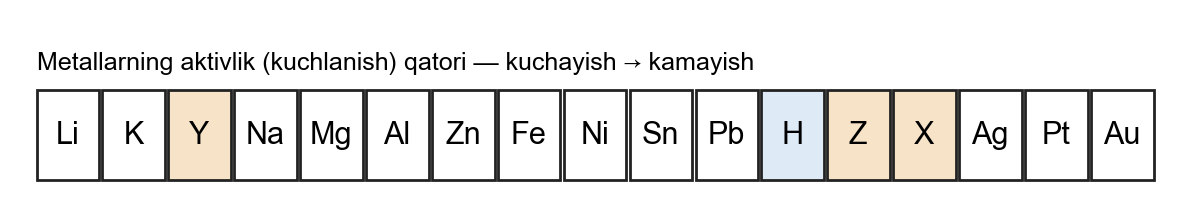
\includegraphics[width=0.86\linewidth]{rasmlar/gen/se_968458.png}\end{center}
\textit{Z} metali tuzining eritmasiga \textit{X} metall plastinka tushirilsa, reaksiya boradimi?
\noindent A)~\textsl{Boradi, \textit{X} faolroq}\par
\noindent B)~\textsl{Faqat qizdirilganda boradi}\par
\noindent C)~\textsl{Faqat konsentrlangan eritmada boradi}\par
\noindent D)~\textsl{Bormaydi, \textit{X} kamroq faol}\par
\qsep
\noindent\qn{15.} D-metallar va ularning birikmalari haqida qaysi fikrlar to`g`ri? 1) Mis nam havoda (CuOH)\textsubscript{2}CO\textsubscript{3} qoplamasi bilan qoplanadi; 2) Cr\textsubscript{2}O\textsubscript{3} asosli oksid; 3) Temirning Cl\textsubscript{2} bilan reaksiyasida FeCl\textsubscript{2} hosil bo`ladi; 4) Cu(OH)\textsubscript{2} qizdirilganda CuO ga parchalanadi

\noindent A)~\textsl{1} \hfill B)~\textsl{1, 2, 4} \hfill C)~\textsl{1, 4} \hfill D)~\textsl{2, 4}\par
\qsep
\noindent\qn{16.} Si va SiO\textsubscript{2} dan iborat 14,8 g aralashma mo`l NaOH eritmasi bilan qizdirilganda 4,48 l (n.sh.) vodorod ajraldi. Reagent (NaOH) eritmasining massa ulushi 10\% va zichligi 1,18 g/ml; u mo`l miqdorda olingan. Aralashmani to`liq eritish uchun sarflangan NaOH \textbf{massasini (g) hisoblang.}

\noindent A)~\textsl{8} \hfill B)~\textsl{16} \hfill C)~\textsl{24} \hfill D)~\textsl{12}\par
\qsep
\noindent\qn{17.} 0,2 mol fosfat kislota 0,5 mol NaOH bilan ta'sirlashtirildi (reagentlar to`liq sarflandi). Hosil bo`lgan tuzlar \textbf{massasini (g) hisoblang.}

\noindent A)~\textsl{30,6} \hfill B)~\textsl{28,4} \hfill C)~\textsl{32,8} \hfill D)~\textsl{61,2}\par
\qsep
\noindent\qn{18.} Oksidlanish darajasi +2 bo`lgan noma'lum \textit{X} metallning oksidi 10\% li sulfat kislota eritmasining stexiometrik miqdorida to`liq eritildi. Hosil bo`lgan tuzning massa ulushi 15,09\% ga teng bo`ldi. \textit{X} \textbf{ni aniqlang.}

\noindent A)~\textsl{Ca} \hfill B)~\textsl{Cu} \hfill C)~\textsl{Ni} \hfill D)~\textsl{Mg}\par
\qsep
\noindent\qn{19.} Na\textsubscript{2}CO\textsubscript{3} va BaCO\textsubscript{3} aralashmasi (101,5 g) mo`l xlorid kislota bilan ta'sirlashganda 15,68 l (n.sh.) gaz ajraldi. Sarflangan HCl \textbf{massasini (g) hisoblang.}

\noindent A)~\textsl{51,1} \hfill B)~\textsl{25,5} \hfill C)~\textsl{102,2} \hfill D)~\textsl{29,2}\par
\qsep
\noindent\qn{20.} Alkanlar va sikloalkanlar haqida qaysi fikrlar to`g`ri? 1) Alkanlar uchun birikish reaksiyalari xos; 2) Alkanlar KMnO\textsubscript{4} eritmasini rangsizlantiradi; 3) Sikloalkanlarning umumiy formulasi CnH\textsubscript{2}n; 4) Metan suvda yaxshi eriydi

\noindent A)~\textsl{2} \hfill B)~\textsl{3, 4} \hfill C)~\textsl{1, 4} \hfill D)~\textsl{3}\par
\qsep
\noindent\qn{21.} Probirkalardagi organik moddalar: fenol, glitserin, etanal ni alohida probirkalarda ajratish uchun qaysi reagent(lar) yetarli? 1) Na metali; 2) FeCl\textsubscript{3}; 3) Cu(OH)\textsubscript{2} (qizdirilganda) va FeCl\textsubscript{3}; 4) Cu(OH)\textsubscript{2} (sovuqda) va FeCl\textsubscript{3}

\noindent A)~\textsl{2, 4} \hfill B)~\textsl{1, 2} \hfill C)~\textsl{3, 4} \hfill D)~\textsl{3}\par
\qsep
\noindent\qn{22.} Quyidagi birikmalardan qaysi biri keton sinfiga kiradi?

\noindent\begin{tabular}{@{}p{0.47\linewidth}@{}p{0.47\linewidth}@{}}
A)~\textsl{CH\textsubscript{3}NO\textsubscript{2}} & B)~\textsl{CH\textsubscript{3}CHO} \\
C)~\textsl{CH\textsubscript{3}COCH\textsubscript{3}} & D)~\textsl{CH\textsubscript{3}COOC\textsubscript{2}H\textsubscript{5}} \\
\end{tabular}\par
\qsep
\noindent\qn{23.} Alkanning monoxlorlanishidan hosil bo`lgan galogenli hosilada xlor massa ulushi 38,4\% ga teng. Dastlabki alkan molekulasidagi uglerod atomlari \textbf{sonini toping.}

\noindent A)~\textsl{5} \hfill B)~\textsl{3} \hfill C)~\textsl{6} \hfill D)~\textsl{4}\par
\qsep
\noindent\qn{24.} 2 mol atsetilen Kucherov reaksiyasi bo`yicha gidratlandi (unum 75\%). Hosil bo`lgan aldegidning 80\% i ammiakli kumush oksid bilan reaksiyaga kirishdi. Barcha reaksiyalar 2 atm bosimda olib borildi. Necha gramm kumush ajraladi?

\noindent A)~\textsl{129,6} \hfill B)~\textsl{518,4} \hfill C)~\textsl{324} \hfill D)~\textsl{259,2}\par
\qsep
\noindent\qn{25.} To`yingan alifatik birlamchi amin yondirilganda hosil bo`lgan CO\textsubscript{2} hajmi azot hajmidan 2 marta ko`p bo`lsa, aminning molyar \textbf{massasini (g/mol) toping.}

\noindent A)~\textsl{45} \hfill B)~\textsl{17} \hfill C)~\textsl{31} \hfill D)~\textsl{48}\par
\qsep
\noindent\qn{26.} 90 g glukoza spirtli bijg`ishga uchradi (unum 75\%). Hosil bo`lgan etanolning yarmi sirka kislotagacha oksidlandi (unum 60\%), qolgan etanol bilan sirka kislota esterlandi (unum 50\%). Hosil bo`lgan murakkab efir \textbf{massasini (g) hisoblang.}

\noindent A)~\textsl{19,8} \hfill B)~\textsl{9,9} \hfill C)~\textsl{4,95} \hfill D)~\textsl{14,85}\par
\qsep
\noindent\qn{27.} Etilen va propendan iborat 18,2 g aralashma mo`l bromli suv bilan to`liq reaksiyaga kirishdi. Xuddi shunday tarkibli ikkinchi porsiya gidratlandi (har bir alken uchun unum 50\%), hosil bo`lgan spirtlar aralashmasi natriy bilan ta'sirlashtirildi. Barcha reaksiyalar 2 atm bosimda olib borildi. Birinchi porsiyada sarflangan brom massasini va ikkinchi porsiyada ajralgan vodorod hajmini (l, n.sh.) \textbf{yig`indisini toping.}

\noindent A)~\textsl{80} \hfill B)~\textsl{82,8} \hfill C)~\textsl{2,8} \hfill D)~\textsl{165,6}\par
\qsep
\noindent\qn{28.} C\textsubscript{3}H\textsubscript{6} dan quyidagi sxema bo`yicha 27,84 g aseton olindi: CH\textsubscript{3}--CH=CH\textsubscript{2} $\to$ CH\textsubscript{3}--CHCl--CH\textsubscript{3} $\to$ CH\textsubscript{3}--CH(OH)--CH\textsubscript{3} $\to$ CH\textsubscript{3}--CO--CH\textsubscript{3}. Bosqichlarning unumi ketma-ket 40\%, 80\%, 60\% ni tashkil qiladi. Barcha reaksiyalar 2 atm bosimda olib borildi. Sarflangan C\textsubscript{3}H\textsubscript{6} hajmi (l, n.sh.) \textbf{ni aniqlang.}

\noindent A)~\textsl{56} \hfill B)~\textsl{112} \hfill C)~\textsl{28} \hfill D)~\textsl{22,4}\par
\qsep
\noindent\qn{29.} 11,2 l (n.sh.) CH\textsubscript{4} dan quyidagi sxema bo`yicha 3,57 g etilen olindi: CH\textsubscript{4} $\to$ CH\textsubscript{3}Cl $\to$ C\textsubscript{2}H\textsubscript{6} $\to$ C\textsubscript{2}H\textsubscript{4}. Dastlabki 2 bosqichning unumi ketma-ket 80\%, 75\% ga teng. Barcha reaksiyalar 1 atm bosimda olib borildi. Oxirgi bosqichning \textbf{unumini (\%) aniqlang.}

\noindent A)~\textsl{42} \hfill B)~\textsl{85} \hfill C)~\textsl{15} \hfill D)~\textsl{68}\par
\qsep
\noindent\qn{30.} Rasmda to`ntarilgan silindrdagi vodorod xlorid gazi suvga tushirilganda suv silindrni to`ldirmoqda. Bu nimani ko`rsatadi?
\begin{center}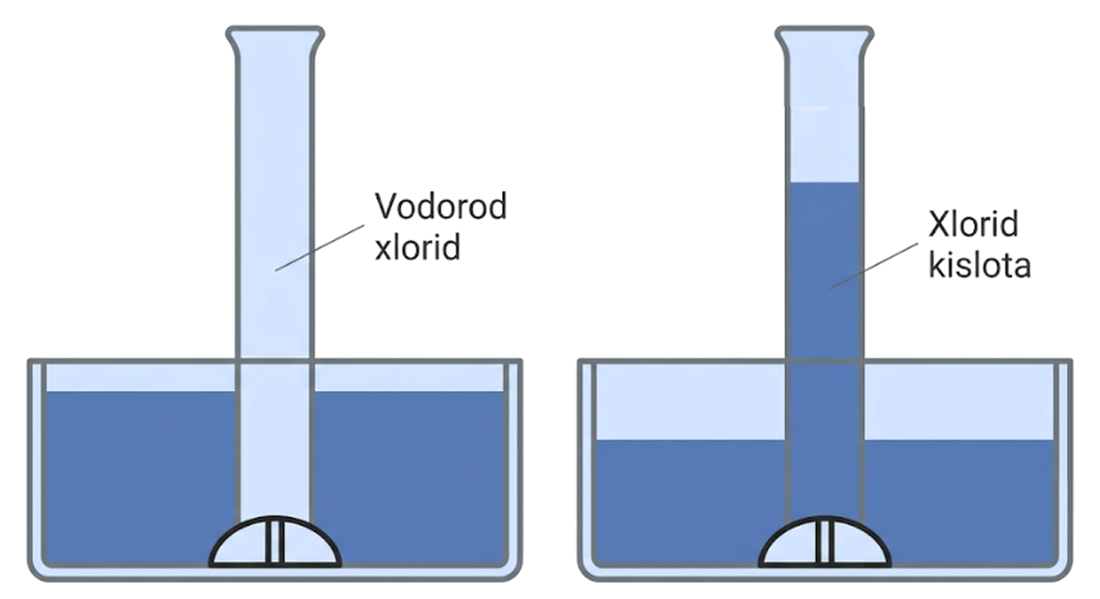
\includegraphics[width=0.86\linewidth]{rasmlar/darslik/d_hcl_erish.png}\end{center}
\noindent A)~\textsl{HCl suv bilan reaksiyaga kirishmaydi}\par
\noindent B)~\textsl{HCl suvda erimaydi}\par
\noindent C)~\textsl{HCl gazi suvda juda yaxshi eriydi}\par
\noindent D)~\textsl{HCl havodan yengil}\par
\qsep
\noindent\qn{31.} Probirkalardagi organik moddalar: etanal, etanol, glitserin ni alohida probirkalarda ajratish uchun qaysi reagent(lar) yetarli? 1) Na metali va FeCl\textsubscript{3}; 2) Cu(OH)\textsubscript{2} (qizdirilganda) va Na metali; 3) [Ag(NH\textsubscript{3})\textsubscript{2}]OH va FeCl\textsubscript{3}; 4) Cu(OH)\textsubscript{2} (sovuqda) va FeCl\textsubscript{3}

\noindent A)~\textsl{2} \hfill B)~\textsl{2, 3} \hfill C)~\textsl{1, 4} \hfill D)~\textsl{1, 2}\par
\qsep
\noindent\qn{32.} 500 g 5\% li eritma tayyorlash uchun 80\% li eritmadan necha gramm olish kerak (qolgani suv)?

\noindent\begin{tabular}{@{}p{0.47\linewidth}@{}p{0.47\linewidth}@{}}
A)~\textsl{31,25} & B)~\textsl{468,75} \\
C)~\textsl{25} & D)~\textsl{62,5   ---} \\
\end{tabular}\par
\qsep
\end{multicols}
\medskip
\noindent\setlength{\fboxsep}{0pt}\fbox{\begin{tabular}{p{0.74\linewidth}|p{0.2\linewidth}}
\parbox[t]{0.72\linewidth}{\vspace{3pt}\textbf{Topshiriqlar (33--35) va javob variant (A--F)larini o`zaro to`g`ri moslashtiring.} Rux va temir qotishmasi (18,6 g) mo`l suyultirilgan H\textsubscript{2}SO\textsubscript{4} da eritilganda 6,72 l (n.sh.) gaz ajraldi; hosil bo`lgan eritmaning hajmi 1000 ml. Eritmaga mo`l NaOH qo`shilib, cho`kma ajratildi, havoda to`liq oksidlanguncha tutildi va doimiy massagacha kuydirildi.
\vspace{3pt}} & \parbox[t]{0.19\linewidth}{\vspace{3pt}A~\textsl{0,2}\\[3pt]
B~\textsl{1,12}\\[3pt]
C~\textsl{8}\\[3pt]
D~\textsl{0,56}\\[3pt]
E~\textsl{0,1}\\[3pt]
F~\textsl{0,08}}\\ \hline
\parbox[t]{0.72\linewidth}{\vspace{2pt}\textbf{33. Eritmada FeSO\textsubscript{4} ning molyar konsentratsiyasini (mol/l) aniqlang.}\vspace{2pt}} & \\ \hline
\parbox[t]{0.72\linewidth}{\vspace{2pt}\textbf{34. Kuydirishdan so`ng qolgan qattiq moddaning massasini (g) toping.}\vspace{2pt}} & \\ \hline
\parbox[t]{0.72\linewidth}{\vspace{2pt}\textbf{35. Cho`kmani oksidlashga sarflangan kislorodning hajmini (l, n.sh.) hisoblang.}\vspace{2pt}} & 
\end{tabular}}
\par\bigskip
\noindent\qn{36.} KMnO\textsubscript{4} + HCl $\to$ MnCl\textsubscript{2} + Cl\textsubscript{2} + KCl + H\textsubscript{2}O reaksiya tenglamasini tenglang va barcha koeffitsiyentlar \textbf{yig`indisini aniqlang.} Tajriba laboratoriyada, kvars idishda o`tkazildi.
\javob\qsep
\noindent\qn{37.} CuCl\textsubscript{2} eritmasi inert elektrodlar yordamida 5 A tok kuchi bilan 965 s elektroliz qilindi. Anodda ajralgan Cl\textsubscript{2} hajmi (l, n.sh.) \textbf{ni toping.}
\javob\qsep
\noindent\qn{38.} Oksidlanish darajasi +2 bo`lgan noma'lum \textit{X} metallning xloridi 5,55 g massada mo`l AgNO\textsubscript{3} eritmasi bilan ta'sirlashganda 14,35 g cho`kma hosil bo`ldi. Reagent (AgNO\textsubscript{3}) eritmasining massa ulushi 50\% va zichligi 1,4 g/ml; u mo`l miqdorda olingan. \textit{X} metallning nisbiy atom \textbf{massasini toping.}
\javob\qsep
\noindent\qn{39.} Vodorodga nisbatan zichligi 22 bo`lgan alkanning 88 g miqdorining 3/4 qismi yorug`likda xlor bilan monoxlorlandi, hosil bo`lgan xloralkan mo`l KOH ning suvli eritmasi bilan gidrolizlandi. Reagent (KOH) eritmasining massa ulushi 20\% va zichligi 1,18 g/ml; u mo`l miqdorda olingan. Hosil bo`lgan spirtning \textbf{massasini (g) toping.}
\javob\qsep
\noindent\qn{40.} 49,2 g nitrobenzol qaytarilib anilin olindi (unum 1/2). Hosil bo`lgan anilinning 3/4 qismi mo`l bromli suv bilan ta'sirlashtirildi. Barcha reaksiyalar 1,5 atm bosimda olib borildi. Hosil bo`lgan cho`kmaning \textbf{massasini (g) toping.}
\javob\qsep
\par\bigskip\begin{center}\textbf{\fontsize{13}{15}\selectfont YOZMA ISH}\end{center}
\noindent\qn{41.} \textbf{Topshiriqni bajarish jarayonida barcha reaksiya tenglamalarini yozing. Miqdoriy va arifmetik hisoblashlarni (unga asos bo`lgan usul yoki formulani ko`rsatgan holda) uzviy ketma-ketlikda bajaring.}\par\smallskip
Tarkibi FeSO\textsubscript{4}$\cdot$nH2O bo`lgan kristallogidratning 11,2 g namunasi suvda eritildi va unga sulfat kislota hamda 25 g 3,4\% li vodorod peroksid eritmasi qo`shildi (H\textsubscript{2}O\textsubscript{2} va H\textsubscript{2}SO\textsubscript{4} qoldiqsiz sarflandi, Fe\textsuperscript{2+} to`liq oksidlandi). Hosil bo`lgan eritmaga mo`l NaOH eritmasi qo`shilib, cho`kma ajratildi va doimiy massagacha kuydirildi. Kuydirish vaqtida ajralgan suv bug`i 127 \textdegree{}C va 83,14 kPa da o`lchandi (R = 8,314 J/(mol$\cdot$K)).\par
\noindent 1)\ Oksidlash, cho`ktirish va kuydirish reaksiyalarining tenglamalarini yozing va tenglashtiring.\par
\noindent 2)\ Kristallogidratdagi n ni aniqlang (tarkibini yozing).\par
\noindent 3)\ Kuydirishdan hosil bo`lgan qattiq moddaning massasini (g) toping.\par
\noindent 4)\ Fe\textsuperscript{3+} ni to`liq cho`ktirish uchun sarflangan NaOH miqdorini (mol) hisoblang.\par
\noindent 5)\ Kuydirishda ajralgan suv bug`ining hajmini (l) aniqlang.\par
\diqqat{Mazkur topshiriq kengaytirilgan javobni talab etib, uning yechilish usuli va shu usul asosidagi barcha hisoblash amallari javoblar varaqasida aks etishi lozim.}\qsep
\noindent\qn{42.} Quyidagi o`zgarishlar zanjirida \textit{X}, \textit{Y}, \textit{Z} noma'lum organik moddalar:\par
\[\setlength{\fboxsep}{0pt}\text{C\textsubscript{2}H\textsubscript{4}Br\textsubscript{2}}\xrightarrow{\text{KOH (spirtli)}}\text{\textit{X}}\xrightarrow{\text{C (aktiv), 600 \textdegree{}C}}\text{\textit{Y}}\xrightarrow{\text{Cl\textsubscript{2}, FeCl\textsubscript{3}}}\text{\textit{Z}}\xrightarrow{\text{NaOH, t\textdegree{}, p}}\text{C\textsubscript{6}H\textsubscript{5}OH}\]
\noindent 1)\ C\textsubscript{2}H\textsubscript{4}Br\textsubscript{2} $\to$ \textit{X} : reaksiya tenglamasini yozing; hosil bo`lgan moddani nomlang.\par
\noindent 2)\ \textit{X} $\to$ \textit{Y} : reaksiya tenglamasini yozing; hosil bo`lgan moddani nomlang.\par
\noindent 3)\ \textit{Y} $\to$ \textit{Z} : reaksiya tenglamasini yozing; hosil bo`lgan moddani nomlang.\par
\noindent 4)\ \textit{Z} $\to$ C\textsubscript{6}H\textsubscript{5}OH : reaksiya tenglamasini yozing; hosil bo`lgan moddani nomlang.\par
\diqqat{Mazkur topshiriq kengaytirilgan javobni talab etib, uning yechilish usuli va shu usul asosidagi barcha hisoblash amallari javoblar varaqasida aks etishi lozim.}\qsep
\noindent\qn{43.} \textbf{Topshiriqni bajarish jarayonida barcha reaksiya tenglamalarini yozing. Miqdoriy va arifmetik hisoblashlarni (unga asos bo`lgan usul yoki formulani ko`rsatgan holda) uzviy ketma-ketlikda bajaring.}\par\smallskip
CaCO\textsubscript{3} va MgCO\textsubscript{3} dan iborat aralashmada ularning massalari nisbati 25 : 14. Aralashma doimiy massagacha qizdirilganda massasi 22 g ga kamaydi. Ajralgan gaz 0,62 mol NaOH saqlagan eritmaga yuttirildi (gaz to`liq yutildi), hosil bo`lgan eritmaga mo`l BaCl\textsubscript{2} eritmasi qo`shildi. Qizdirishdan qolgan qattiq qoldiq esa 10\% li xlorid kislotaning stexiometrik miqdorida eritildi. Qoldiqning HCl dagi eritmasiga mo`l Na\textsubscript{2}CO\textsubscript{3} eritmasi qo`shilib, hosil bo`lgan cho`kma ajratildi va doimiy massagacha qizdirildi; ajralgan gaz mo`l ohakli suvga yuborildi.\par
\noindent 1)\ Barcha reaksiyalarning tenglamalarini yozing va tenglashtiring. Dastlabki aralashmadagi karbonatlarning massalarini (g) aniqlang.\par
\noindent 2)\ Ajralgan gazning hajmini (l, n.sh.) hisoblang va hosil bo`lgan tuzlar tarkibini (o`rta/nordon) aniqlang.\par
\noindent 3)\ Gaz yutilgandan keyingi eritmadagi tuzlarning massalarini (g) toping. Na\textsubscript{2}CO\textsubscript{3} qo`shilganda hosil bo`lgan cho`kmalarning umumiy massasini (g) hisoblang.\par
\noindent 4)\ BaCl\textsubscript{2} qo`shilganda hosil bo`lgan cho`kma massasini (g) hisoblang. Cho`kma qizdirilganda massa necha gramga kamayadi?\par
\noindent 5)\ Qoldiq erigan eritmaning massasini (g) va undagi tuzlarning massa ulushlarini (\%) toping. Ohakli suvga yuborilganda hosil bo`lgan cho`kma massasini (g) toping.\par
\diqqat{Mazkur topshiriq kengaytirilgan javobni talab etib, uning yechilish usuli va shu usul asosidagi barcha hisoblash amallari javoblar varaqasida aks etishi lozim.}\qsep
\newpage
\noindent\textbf{\fontsize{13}{15}\selectfont 1-variant}\hfill \textbf{Javoblar kaliti}\par\smallskip\hrule\smallskip
\textit{Faqat o`qituvchi uchun.}\par\medskip
\noindent\textbf{1--32-savollar}\par\smallskip
\noindent\begin{tabular}{|c|c|c|c|c|c|c|c|c|c|c|c|c|c|c|c|}\hline
\textbf{1} & \textbf{2} & \textbf{3} & \textbf{4} & \textbf{5} & \textbf{6} & \textbf{7} & \textbf{8} & \textbf{9} & \textbf{10} & \textbf{11} & \textbf{12} & \textbf{13} & \textbf{14} & \textbf{15} & \textbf{16}\\\hline
\textsl{D} & \textsl{B} & \textsl{C} & \textsl{A} & \textsl{C} & \textsl{D} & \textsl{D} & \textsl{B} & \textsl{B} & \textsl{A} & \textsl{D} & \textsl{B} & \textsl{A} & \textsl{D} & \textsl{C} & \textsl{C}\\\hline
\textbf{17} & \textbf{18} & \textbf{19} & \textbf{20} & \textbf{21} & \textbf{22} & \textbf{23} & \textbf{24} & \textbf{25} & \textbf{26} & \textbf{27} & \textbf{28} & \textbf{29} & \textbf{30} & \textbf{31} & \textbf{32}\\\hline
\textsl{A} & \textsl{B} & \textsl{A} & \textsl{D} & \textsl{C} & \textsl{C} & \textsl{D} & \textsl{D} & \textsl{C} & \textsl{B} & \textsl{B} & \textsl{A} & \textsl{B} & \textsl{C} & \textsl{A} & \textsl{A}\\\hline
\end{tabular}\par\medskip
\noindent\textbf{33--35-savollar}\par\smallskip
\noindent\begin{tabular}{|c|c|c|}\hline \textbf{No} & \textbf{Javob} & \textbf{Qiymat}\\\hline
33 & \textsl{E} & 0,1\\\hline
34 & \textsl{C} & 8\\\hline
35 & \textsl{D} & 0,56\\\hline
\end{tabular}\par\medskip
\noindent\textbf{36--40-savollar}\par\smallskip
\noindent\begin{tabular}{|c|c|}\hline \textbf{No} & \textbf{To`g`ri javob}\\\hline
36 & 35\\\hline
37 & 0,56\\\hline
38 & 40\\\hline
39 & 90\\\hline
40 & 49,5\\\hline
\end{tabular}\par\medskip
\noindent\textbf{41--43-topshiriqlar: javoblar}\par\smallskip
\noindent\textbf{41-topshiriq.}\par
\noindent 1) 2FeSO\textsubscript{4} + H\textsubscript{2}O\textsubscript{2} + H\textsubscript{2}SO\textsubscript{4} $\to$ Fe\textsubscript{2}(SO\textsubscript{4})\textsubscript{3} + 2H\textsubscript{2}O; Fe\textsubscript{2}(SO\textsubscript{4})\textsubscript{3} + 6NaOH $\to$ 2Fe(OH)\textsubscript{3}$\downarrow$ + 3Na\textsubscript{2}SO\textsubscript{4}; 2Fe(OH)\textsubscript{3} $\to$ Fe\textsubscript{2}O\textsubscript{3} + 3H\textsubscript{2}O (t)\par
\noindent 2) FeSO\textsubscript{4}$\cdot$4H\textsubscript{2}O\par
\noindent 3) 4 g\par
\noindent 4) 0,15 mol\par
\noindent 5) 3 l\par
\noindent\textbf{42-topshiriq.}\par
\noindent 1) C\textsubscript{2}H\textsubscript{4}Br\textsubscript{2} + KOH (spirtli) $\to$ C\textsubscript{2}H\textsubscript{2} (asetilen)\par
\noindent 2) C\textsubscript{2}H\textsubscript{2} + C (aktiv), 600 \textdegree{}C $\to$ C\textsubscript{6}H\textsubscript{6} (benzol)\par
\noindent 3) C\textsubscript{6}H\textsubscript{6} + Cl\textsubscript{2}, FeCl\textsubscript{3} $\to$ C\textsubscript{6}H\textsubscript{5}Cl (xlorbenzol)\par
\noindent 4) C\textsubscript{6}H\textsubscript{5}Cl + NaOH, t\textdegree{}, p $\to$ C\textsubscript{6}H\textsubscript{5}OH (fenol)\par
\noindent\textbf{43-topshiriq.}\par
\noindent 1) 30 g; 16,8 g\par
\noindent 2) 11,2 l\par
\noindent 3) 13,25 g; 31,5 g; 46,8 g\par
\noindent 4) 24,62 g; 22 g\par
\noindent 5) 389,8 g; 8,54\%; 4,87\%; 50 g\par
\par\bigskip\noindent\textbf{Mavzular taqsimoti}\par\smallskip
{\small\noindent\begin{longtable}{|c|p{7.2cm}|p{5.4cm}|c|}\hline \textbf{No} & \textbf{Mavzu} & \textbf{Tekshiriladigan ko`nikma} & \textbf{Ball}\\\hline
1 & 8-sinf (izotoplar, izobarlar, jadval) & Jadval tahlili & 1\\\hline
2 & 8-sinf; Tirkashev \textit{V} bob (oksidlanish darajasi) & Bilim va tushunish & 1\\\hline
3 & 10-sinf \S{}17 & Bilim va tushunish & 1\\\hline
4 & Tirkashev I bob; 8-sinf (izoelektron) & Bilim va tushunish & 1\\\hline
5 & Tirkashev I bob; 8-sinf (elektron konfiguratsiya) & Bilim va tushunish & 1\\\hline
6 & 8-9-sinf (eritmalar; ketma-ket jarayon) & Hisoblash va masala yechish & 1\\\hline
7 & 8-sinf (havo tarkibi, diagramma) & Grafik tahlili & 1\\\hline
8 & 9-sinf; 11-sinf (tuzlar gidrolizi; Le-Shatelye) & Bilim va tushunish & 1\\\hline
9 & 9-sinf (metallarning kislotalar bilan reaksiyasi) & Hisoblash va masala yechish & 1\\\hline
10 & Tirkashev III bob (kristallogidrat) & Hisoblash va masala yechish & 1\\\hline
11 & Tirkashev VI bob (muvozanat, jadval) & Jadval tahlili & 1\\\hline
12 & Tirkashev VI bob (Le-Shatelye) & Bilim va tushunish & 1\\\hline
13 & Tirkashev \textit{V} bob; Tashev (HNO\textsubscript{3}, H\textsubscript{2}SO\textsubscript{4}) & Hisoblash va masala yechish & 1\\\hline
14 & 9-sinf (metallar aktivligi) & Rasm bo`yicha tahlil & 1\\\hline
15 & 9-sinf; Tashev (Fe, Cu, Zn, Cr) & Bilim va tushunish & 1\\\hline
16 & 9-sinf (kremniy va uning oksidi) & Hisoblash va masala yechish & 1\\\hline
17 & 9-sinf (ko`p negizli kislotalar, nordon tuzlar) & Hisoblash va masala yechish & 1\\\hline
18 & 9-sinf (oksidlar; eritma massa ulushi) & Hisoblash va masala yechish & 1\\\hline
19 & 8-9-sinf (karbonatlar; kislotalar bilan reaksiya) & Hisoblash va masala yechish & 1\\\hline
20 & 10-sinf (mavzuga oid paragraflar); Abdusamatov & Bilim va tushunish & 1\\\hline
21 & 10-sinf (spirt, aldegid, fenol sifat reaksiyalari) & Bilim va tushunish & 1\\\hline
22 & 10-sinf (organik birikmalar sinflari) & Bilim va tushunish & 1\\\hline
23 & 10-sinf (alkan va alkenlarning galogenli hosilalari) & Hisoblash va masala yechish & 1\\\hline
24 & 10-sinf (alkinlar, aldegidlar) & Hisoblash va masala yechish & 1\\\hline
25 & 10-sinf (aminlar yonishi) & Hisoblash va masala yechish & 1\\\hline
26 & 10-sinf (uglevodlar, spirtlar, kislotalar, efirlar) & Hisoblash va masala yechish & 1\\\hline
27 & 10-sinf (alkenlar: birikish, gidratlanish; spirtlar + Na) & Hisoblash va masala yechish & 1\\\hline
28 & 10-sinf (alkenlar, galogenli hosilalar, spirtlar) & Hisoblash va masala yechish & 1\\\hline
29 & 10-sinf (alkanlar; Vyurs reaksiyasi; degidrogenlash) & Hisoblash va masala yechish & 1\\\hline
30 & 8-sinf (19-rasm) & Rasm bo`yicha tahlil & 1\\\hline
31 & 10-sinf (spirt, aldegid, fenol sifat reaksiyalari) & Bilim va tushunish & 1\\\hline
32 & Tirkashev III bob (eritma tayyorlash) & Hisoblash va masala yechish & 1\\\hline
33--35 & Aralash masala (moslashtirish) & Ko`p bosqichli hisob & 3\\\hline
36--40 & Qisqa javobli masalalar & Hisoblash & 5\\\hline
41--43 & Yozma ish & Usul va hisob (M, A) & 75\\\hline
\end{longtable}}
\end{document}
